\documentclass[a4paper, english, 12pt, reqno, draft]{amsart}

% ---------------------------------------------------------------------------

% Usepackages recommended in mcom-l-template.tex if needed.

\usepackage{amssymb}
% \usepackage{graphicx}
% \usepackage[cmtip,all]{xy}

% ---------------------------------------------------------------------------

% Usepackages inserted by authors.

\usepackage[english]{babel}
\usepackage[utf8]{inputenc}
\usepackage{tikz,tikzscale}
\tikzset{>=latex}
\usepackage{xcolor}
\usepackage{enumerate}
\usepackage{booktabs,multirow}
\usepackage{amsfonts}

%%%%%%%%%% Packages to help editing %%%%%%%%%%
\usepackage[notref,notcite]{showkeys} % Show labels.
\usepackage[mode=multiuser]{fixme} % Provide note, warning, error, fatal.
\FXRegisterAuthor{gk}{envgk}{GK}
\FXRegisterAuthor{ar}{envar}{AR}
\fxusetheme{color}

% ---------------------------------------------------------------------------

% Theorems in the AMS style.

\newtheorem{theorem}{Theorem}[section]
\newtheorem{lemma}[theorem]{Lemma}
\newtheorem{corollary}[theorem]{Corollary}

\theoremstyle{definition}
\newtheorem{definition}[theorem]{Definition}
\newtheorem{example}[theorem]{Example}
\newtheorem{exercise}[theorem]{Exercise}

\theoremstyle{remark}
\newtheorem{remark}[theorem]{Remark}

\numberwithin{equation}{section}

% ---------------------------------------------------------------------------

% Newcommands by the authors.

\newcommand{\graph}{\ensuremath{\mathcal G}}
\newcommand{\setEdge}{\ensuremath{\mathcal E}}
\newcommand{\setNode}{\ensuremath{\mathcal N}}
\newcommand{\edge}{\ensuremath{E}}
\newcommand{\node}{\ensuremath{N}}
\newcommand{\locDim}{\ensuremath{\mathfrak d}}
\newcommand{\globDim}{\ensuremath{\mathfrak D}}

\newcommand{\IN}{\ensuremath{\mathbb N}}
\newcommand{\IR}{\ensuremath{\mathbb R}}

\newcommand{\elem}{\ensuremath{T}}
\newcommand{\mesh}{\ensuremath{\mathcal T}}
\newcommand{\meshIndex}{\ensuremath{\mathcal I}}
\newcommand{\faceSet}{\ensuremath{\mathcal F}}
\newcommand{\faceSetDir}{\ensuremath{\mathcal F^\textup D}}
\newcommand{\face}{\ensuremath{F}}
\newcommand{\skeletal}{\ensuremath{\Sigma}}
\newcommand{\skeletalSpace}{\ensuremath{M}}
\newcommand{\skeletalSpaceHDG}{\ensuremath{M}}
\newcommand{\contElementSpace}{\ensuremath{V^\textup c}}
\newcommand{\contThreeElementSpace}[1]{\ensuremath{V^\textup c_{#1,p+3}}}
\newcommand{\linElementSpace}{\ensuremath{\overline V^\textup c}}
\newcommand{\discElementSpace}{\ensuremath{V}}
\newcommand{\polynomials}{\ensuremath{\mathcal P}}
\newcommand{\level}{\ensuremath{\ell}}
\newcommand{\iterMgOuter}{i}%\ensuremath{\nu}}
\newcommand{\iterMgInner}{m}%\ensuremath{\eta}}

\newcommand{\Div}{\nabla\!\cdot\!}
\newcommand{\discLaplacian}{\ensuremath{A}}
\newcommand{\extensionOp}{\ensuremath{\mathcal U^\textup c}}
\newcommand{\averagingOp}{\ensuremath{I^\textup{avg}}}
\newcommand{\restrictionOp}{\ensuremath{I^\textup{res}}}
\newcommand{\traceOp}{\ensuremath{\gamma_0}}
\newcommand{\injectionOp}{\ensuremath{I}}
\newcommand{\projectionOp}{\ensuremath{P}}
\newcommand{\projectionOrthogonalOP}{\ensuremath{\Pi}}
\newcommand{\projectionLinOp}{\ensuremath{\overline P}}
\newcommand{\skeletalProj}{\ensuremath{\Pi^\partial}}
\newcommand{\contLinProj}{\ensuremath{\overline \Pi^\textup c}}
\newcommand{\discProj}{\ensuremath{\Pi^\textup d}}
\newcommand{\liftingOp}{\ensuremath{S}}

\renewcommand{\vec}[1]{\ensuremath{\boldsymbol{#1}}}
\newcommand{\Nu}{\ensuremath{\vec \nu}}
\newcommand{\dx}{\ensuremath{\, \textup d x}}
\newcommand{\ds}{\ensuremath{\, \textup d \sigma}}
\newcommand{\localU}{\ensuremath{\mathcal U}}
\newcommand{\localQ}{\ensuremath{\vec{\mathcal Q}}}
\newcommand{\penaltyParam}{\ensuremath{\eta}}

\newcommand{\tildelambda}{\tilde\lambda}
\newcommand{\ureconstructed}{\overline{u}}
\newcommand{\projectionBramble}{\ensuremath{\bar B}}
\newcommand{\indexDOF}{\ensuremath{i}}
\newcommand{\IndexDOF}{\ensuremath{\mathcal I}}

\newcommand{\llangle}{\ensuremath{\langle \! \langle}}
\newcommand{\rrangle}{\ensuremath{\rangle \! \rangle}}
\newcommand{\nnorm}{\ensuremath{\vert \! \vert \! \vert}}

% ---------------------------------------------------------------------------

% Make paragraph heading being small capitals!

\makeatletter
\def\paragraph{\@startsection{paragraph}{4}%
  \z@\z@{-\fontdimen2\font}%
  {\normalfont\scshape}}
\makeatother

% ---------------------------------------------------------------------------

% Usepackage hyperref is the last to be added!

\usepackage[colorlinks = true, linkcolor = blue, citecolor = blue, urlcolor = blue]{hyperref}

% ---------------------------------------------------------------------------

% Document head as described in the template.

\begin{document}

\title[H\MakeLowercase{yper}HDG]{H\MakeLowercase{yper}HDG --- Hybrid disontinuous Galerkin methods for PDEs on hypergraphs} 

\author{Andreas Rupp}
\address{Interdisciplinary Center for Scientific Computing (IWR), Heidelberg University, Mathematikon, Im Neuenheimer Feld 205, 69120 Heidelberg, Germany}
% \curraddr{}
\email{andreas.rupp@fau.de, andreas.rupp@uni-heidelberg.de}
\thanks{This work is supported by the Deutsche Forschungsgemeinschaft (DFG, German Research Foundation) under Germany's Excellence Strategy EXC 2181/1 - 390900948 (the Heidelberg STRUCTURES Excellence Cluster).}

\author{Guido Kanschat}
\address{Interdisciplinary Center for Scientific Computing (IWR) and Mathematics Center Heidelberg (MATCH), Heidelberg University, Mathematikon, Im Neuenheimer Feld 205, 69120 Heidelberg, Germany}
% \curraddr{}
\email{kanschat@uni-heidelberg.de}
% \thanks{}

\subjclass[2010]{\textcolor{red}{TODO}}

\date{\today}

% \dedicatory{}

\begin{abstract}
 \textcolor{red}{\textsc{Todo!}} 
 \\[1ex] \noindent \textsc{Keywords.}
 \textcolor{red}{TODO!}
\end{abstract}
% 
\maketitle
% 
\section{Introduction}
% 
% ---------------------------------------------------------------------
\section{Hypergraphs}\label{SEC:hypergraph}
% ---------------------------------------------------------------------
% 
HyperHDG is a simumlation software to perform numerical experiments on so called hypergraphs. To this end, it is useful to discuss the composition of hypergraphs in some detail. At first, every hypergraph is defined as topological hypergraph, cf. Section. \ref{SEC:hypergraph_topology}. Additionally, a hypergraph may be equipped with a geometry, as illuminated in Section \ref{SEC:hypergraph_geometry}. 
% 
\subsection{Topologic aspects of hypergraphs}\label{SEC:hypergraph_topology}
% 
In the whole manuscript, we consider a \emph{hypergraph} $\graph = (\setNode,\setEdge)$ consisting of a finite set of \emph{hypernodes} $\setNode = \{\node_1, \node_2, \ldots \}$ and a set of \emph{hyperedges} $\setEdge = \{\edge_1, \edge_2, \ldots \}$. All hyperedges $\edge \in \setEdge$ can be interpreted as connecting several nodes and, thus, can be written as $\edge \subset \setNode$.

Thus, the topology of a hypergraph is a $\graph$ is a pair consisting a set of hyperedges $\setEdge$ and a set of hypernodes $\setNode$. Each hypernodes $\edge \in \setEdge$ is connected to other hypernodes via the set of its adjacent hypernodes. Note that this is exactly the inverted interpretation as compared to standard graph theory, where nodes are interpreted as connected via edges.

\paragraph{Cubic and simplicial hypergraphs, and local dimension $\locDim$}
% 
We will define partial differential equations (PDEs) on hypergraphs. To do so, it helps---but is not necessary---to have an adequate graphical representation of hyperedges. For example, one might try to represent all $\edge \in \setEdge$ as open hypercubes of dimension $\locDim \in \IN$. A hypergraph, of which all hypereges $\edge = \{ \node_1, \node_2, \ldots, \node_{2\locDim} \}$ consist of exactly $2\locDim$ hypernodes, allows for such a representation of all hyperedges. The hypernodes may then be interpreted as the \emph{faces} (not the vertices) of the hypercubes/hyperedges and the hypergraph is denoted \emph{cubic} of \emph{local dimension} $\locDim$.

Analogously, a hypergraph of which all hyperedges consist of $\locDim+1$ is called simplicial of local dimension $\locDim$.

\paragraph{Cubic/simplicial embeddings of hypergraphs to global dimension $\globDim$}
% 
If one wants to represent the whole hypergraph at once (instead of only single hyperedges), an embeddind to an $\globDim$ dimensional space is needed. A cubic/simplicial hypergraph can be embedded into $\IR^\globDim$ if there is a way to assemble all hypercubes/simplices (representing the hyperedges) such that for two hyperedges $\edge^+ \neq \edge^-$, we have $\edge^- \cap \edge^+ = \emptyset$.

If additionally for two hypernodes $\node^+ \neq \node^-$ the intersection of their interiors is empty, the hypergraph is denoted \emph{regularly cubic/simplicial embeddable} to dimension $\globDim$.

\paragraph{Examples for cubic hypergraphs}
% 
According to this definition, every graph is both a cubic and a simplicial hypergraph. An illustration which can be interpreted as several hypergraphs---all regularly embedded to $\globDim = 3$---can be found in Figure \ref{FIG:hyG_topo}:
% 
\begin{itemize}
 \item Cubic or simplicial hypergraph of $\locDim = 1$ consisting of twelve hypernodes (vertices) and  twenty hyperedges (lines).
 \item Cubic hypergraph of $\locDim = 2$ consisting of twenty hypernodes (lines) and eleven hyperedges (squares).
 \item Cubic hypergraph of $\locDim = 3$ consisting of two eleven hypernodes (squares) and two hyperedges (cubes).
\end{itemize}
% 
\begin{figure}[ht]
 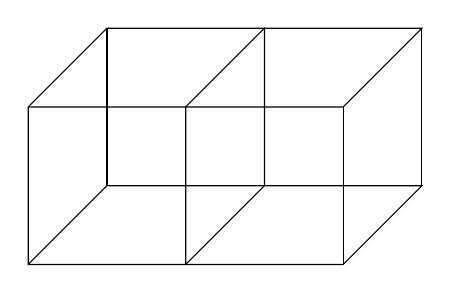
\begin{tikzpicture}
  \draw (0,0) -- (2,0) -- (4,0) -- (5,1) -- (3,1) -- (1,1) -- (0,0) -- (0,2) -- (2,2) -- (4,2) -- (5,3) -- (3,3) -- (1,3) -- (0,2);
  \draw (2,0) -- (3,1) -- (3,3) -- (2,2) -- (2,0);
  \draw (1,1) -- (1,3);
  \draw (4,0) -- (4,2);
  \draw (5,1) -- (5,3);
 \end{tikzpicture}
 \caption{Illustration that can be interpreted as several types of hypergraph topologies.}\label{FIG:hyG_topo}
\end{figure}
% 
\subsection{Geometrical aspects of hypergraphs}\label{SEC:hypergraph_geometry}
% 
Figure \ref{FIG:hyG_topo} already indicates that hypergraphs, especially those with (regular) embeddings might be equipped with geometrical information. This specific example indicates that all lines, squares, cubes are of unit size. However, the hypergraph might also have geometrical information that says it looks like in Figure \ref{FIG:hyG_geom}, where the first picture is valid for all $\locDim$ and the second one is only valid for $\locDim = 3$.
% 
\begin{figure}[ht]
 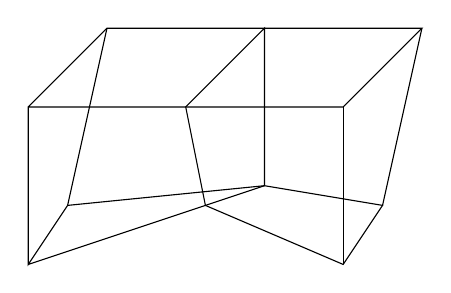
\begin{tikzpicture}
  \draw (0,0) -- (2.25,0.75) -- (4,0) -- (4.5,0.75) -- (3,1) -- (0.5,0.75) -- (0,0) -- (0,2) -- (2,2) -- (4,2) -- (5,3) -- (3,3) -- (1,3) -- (0,2);
  \draw (2.25,0.75) -- (3,1) -- (3,3) -- (2,2) -- (2.25,0.75);
  \draw (0.5,0.75) -- (1,3);
  \draw (4,0) -- (4,2);
  \draw (4.5,0.75) -- (5,3);
 \end{tikzpicture}
 \quad
  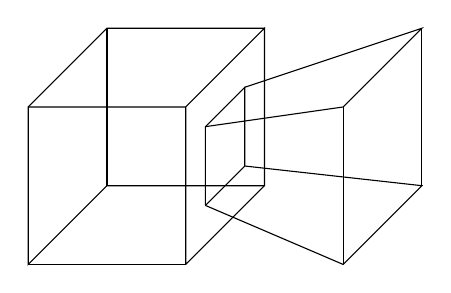
\begin{tikzpicture}
  \draw (0,0) -- (2,0);
  \draw (2.25,0.75)  -- (4,0) -- (5,1) -- (2.75,1.25);
  \draw (3,1) -- (1,1) -- (0,0) -- (0,2) -- (2,2);
  \draw (2.25,1.75) -- (4,2) -- (5,3) -- (2.75,2.25); 
  \draw (3,3) -- (1,3) -- (0,2);
  \draw (2,0) -- (3,1) -- (3,3) -- (2,2) -- (2,0);
  \draw (2.25,0.75) -- (2.75,1.25) -- (2.75,2.25) -- (2.25,1.75) -- (2.25,0.75);
  \draw (1,1) -- (1,3);
  \draw (4,0) -- (4,2);
  \draw (5,1) -- (5,3);
 \end{tikzpicture}
 \caption{Two possible geometrical representation of the hypergraph in Figure \ref{FIG:hyG_topo}. The second one is only valid for $\locDim = 3$.}\label{FIG:hyG_geom}
\end{figure}


% 
% ---------------------------------------------------------------------
\section{Model equation and discretization}\label{SEC:basics}
% ---------------------------------------------------------------------
% 
We consider the standard diffusion equation in mixed form defined on a polygonally bounded Lipschitz domain $\Omega \subset \mathbb R^d$ with boundary $\partial \Omega$. We assume homogeneous Dirichlet boundary conditions on $\partial\Omega$. Thus, we approximate solutions $(u, \vec q)$ of
% 
\begin{subequations}\label{EQ:diffusion_mixed}
\begin{align}
 \Div \vec q & = f && \text{ in } \Omega,\\
 \vec q + \nabla u & = 0 && \text{ in } \Omega,\\
 u & = 0 && \text{ on } \partial \Omega,%\\
%  \vec q \cdot \Nu & = g_\text N && \text{ on } \Gamma_\text N,
\end{align}
\end{subequations}
% 
for a given function $f$. Here, and in the following, $L^2(\Omega)$ denotes the space of square integrable functions on $\Omega$ with inner product and norm
\begin{equation}
 (u,v)_0 := \int_\Omega u v \dx, \qquad \text{and} \qquad \| u \|^2_0 := (u,u)_0.
\end{equation}
%
The space $H^k(\Omega)$ is the Sobolev space of $k$-times weakly
differentiable functions with derivatives in $L^2(\Omega)$.
% 
% ---------------------------------------------------------------------
\subsection{Spaces for the HDG on hypergraphs}
% ---------------------------------------------------------------------
%
Starting out from a subdivision $\graph = (\setEdge, \setNode)$.

By $\faceSet$ we denote the set of faces of $\mesh_\level$.
The subset of faces on the boundary is
\begin{gather}
  \faceSetDir_\level := \{\face \in \faceSet_\level : \face \subset \partial \Omega \}.
\end{gather}
Moreover, we define
$\faceSet^\elem_\level := \{ \face \in \faceSet_\level : \face \subset
\partial \elem \}$ as the set of faces of a cell $\elem\in\mesh_\level$.  On the set of faces, we define the space $L^2(\faceSet_\ell)$ as the space of
square integrable functions with the inner product
\begin{gather}
  \llangle \lambda, \mu \rrangle_\level = \sum_{\elem \in \mesh_\level} \int_{\partial \elem} \lambda\mu\ds,
\end{gather}
and its induced norm
$\nnorm \mu \nnorm^2_\level = \llangle \mu, \mu
\rrangle_\level$. Note that interior faces appear twice in this definition such that expressions like $\llangle u, \mu \rrangle_\level$ with possibly discontinuous $u|_{\elem} \in H^1(\elem)$ for all $\elem \in \mesh_\level$ and $\mu \in L^2(\faceSet)$ are defined without further ado. Additionally, we define an inner product
commensurate with the $L^2$-inner product in the bulk domain, namely
\begin{gather}
  \langle \lambda, \mu \rangle_\level
  = \sum_{\elem \in \mesh_\level} \frac{|\elem|}{|\partial \elem|}
  \int_{\partial \elem} \lambda \mu \ds \cong \sum_{\face \in \faceSet_\level} h_\face
  \int_{\face} \lambda \mu \ds.
\end{gather}
Its induced norm is $ \| \mu \|^2_\level = \langle \mu, \mu \rangle_\level$.

Let $p\ge 1$ and $\polynomials_p$ be the space of (multivariate)
polynomials of degree up to $p$. Then, we define the space of piecewise
polynomials on the skeleton by
\begin{gather}
  \label{EQ:skeletal_space}
  \skeletalSpace_\level := \left\{ \lambda \in L^2(\faceSet_\level) \;\middle|\;
    \begin{array}{r@{\,}c@{\,}ll}
  \lambda_{|\face} &\in& \polynomials_p & \forall \face \in \faceSet_\level\\
  \lambda_{|\face} &=& 0 & \forall \face \in \faceSetDir_\level    
    \end{array}
  \right\}.
\end{gather}

The HDG method involves a local solver on each mesh cell
$\elem \in \mesh_\level$, producing cellwise approximations $u_\elem \in V_\elem$
and and $\vec q_\elem\in \vec W_\elem$ of the functions $u$ and $\vec q$ in
equation~\eqref{EQ:diffusion_mixed}, respectively. We choose
$V_\elem = \polynomials_p$. Then, choosing
$\vec W_\elem = \polynomials_p^d$ yields the so called hybridizable local discontinuous Galerkin (LDG-H) scheme. Our current analysis is in fact limited to this case and other choices require a modification of Lemma~\ref{LEM:u_q_bound}. We will also use the concatenations of the spaces $V_\elem$
and $\vec W_\elem$, respectively, as a function space on $\Omega$, namely
\begin{gather}
  \label{EQ:dg_spaces}
  \begin{aligned}
    \discElementSpace_\level
    &:=\bigl\{ v \in L^2(\Omega)
    & \big|\;v_{|\elem} &\in V_\elem,
    &\forall \elem &\in \mesh_\level \bigr\},\\
    \vec W_\level
    &:=\bigl\{ \vec q \in L^2(\Omega;\mathbb R^d)
    & \big|\;\vec q_{|\elem} &\in \vec W_\elem,
    &\forall \elem &\in \mesh_\level \bigr\}.    
  \end{aligned}
\end{gather}
%\begin{alignat}2
% \end{alignat}



% 
\bibliographystyle{alpha}
\bibliography{HyperHDG}
% 
\end{document}
